%\documentclass[preprint,tightenlines,showpacs,showkeys,floatfix,
%nofootinbib,superscriptaddress,fleqn]{revtex4} 
\documentclass[tightenlines,floatfix,nofootinbib,superscriptaddress,fleqn]{revtex4} 
%\documentclass[aps,epsfig,tightlines,fleqn]{revtex4}
\usepackage{kotex}
\usepackage[HWP]{dhucs-interword}
\usepackage[dvips]{color}
\usepackage{graphicx}
\usepackage{bm}
%\usepackage{fancyhdr}
%\usepackage{dcolumn}
\usepackage{defcolor}
\usepackage{amsmath}
\usepackage{amsfonts}
\usepackage{amssymb}
\usepackage{amscd}
\usepackage{amsthm}
\usepackage[utf8]{inputenc}
%\pagestyle{fancy}
\begin{document}

\title{\Large 2022년 2학기 물리학 II}
\author{김현철\footnote{Office: 5S-436D (면담시간 매주
    수요일-16:15$\sim$18:00)}} 
\email{hchkim@inha.ac.kr}
\affiliation{Hadron Theory Group, Department of Physics,
  Inha University, Incheon 22212, Republic of Korea }
\date{Autumn Semester, 2022}

\maketitle

{\color{red} {\bf Due date:} 2022년 8월 31일  15:30-16:15 }
\vspace{1.cm}


{\bf 학번:} \hspace{4cm}
{\bf 이름:} 

\section*{\large Quiz 2}
\noindent {\bf 문제 1 [20pt].}
반지름이 $a$인 원형고리가 원점을 중심으로 $x-y$ 평면에 놓여 있다.  
이 중심에서부터 $z$축으로 $z$만큼 떨어진 $P$점에서 이 원형고리가
생성시키는 전기장의 크기와 방향을 구하려고 한다.
\begin{itemize}
\item 원점에서부터 원형고리를 따라 있는 미소길이 $ds$까지의 거리 벡터
  $\vec{r}'$을 구하여라. 
\item 원점에서부터 $P$점까지 거리 벡터 $\vec{r}$을 구하여라.
\item $|\vec{r}-\vec{r}'|$을 구하여라. 

\item 위 문제에 대한 전기장을 표현하여라.
\item $P$점에서 전기장을 구하여라. 
\item 결과를 토론하여라. (예: 전기장의 방향은 왜 $z$축 방향만 있는가?
  $z\gg a$ 일 때 전기장은? 등등)  
\end{itemize}

\newpage
{\color{gray} [문제 풀이 쪽]}
\newpage
\noindent {\bf 문제 2 [5pt].}크기가 $1.00\times 10^3$ N/C인 균일한
전기장 안에 전자를 가만히 놓았다. 전자가 1.00 cm를 진행했을 때,
\begin{itemize}
\item[(가)] 전자의 속력은 얼마인가? 
\item[(나)] 전자의 운동에너지는 얼마인가? 
\item[(다)] 시간은 얼마나 지났는가? 
\end{itemize}
\newpage
{\color{gray} [문제 풀이 쪽]}
\newpage

\noindent {\bf 문제 3 [10pt].} 그림~\ref{fig:1}처럼 각각 전하가 $q$,
$-q$인 두 입자가 전기 쌍극자를 이루고 있다. $x\gg a$일 때 $x$ 축
위에서 전기장 $E_x$를 구하여라. 
\begin{figure}[htp]
  \centering
  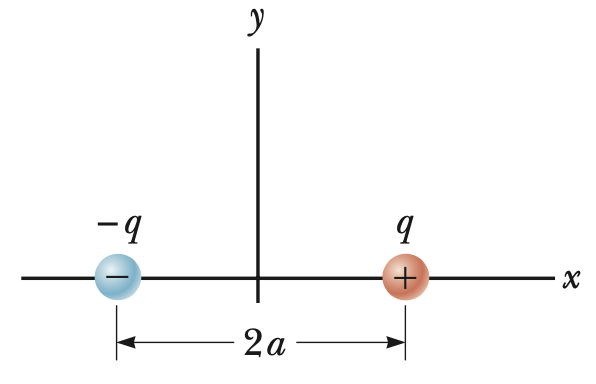
\includegraphics[scale=0.6]{qfig2-1.png}
  \caption{\textbf{문제 1}}
  \label{fig:1}
\end{figure}
\newpage
{\color{gray} [문제 풀이 쪽]}
\newpage

\noindent {\bf 문제 4 [10pt].} 그림~\ref{fig:2}처럼 한 변의 길이가
$a$인 정사각형의 꼭짓점에 네 개의 전하가 각각 놓여있다.
\begin{figure}[htp]
  \centering
  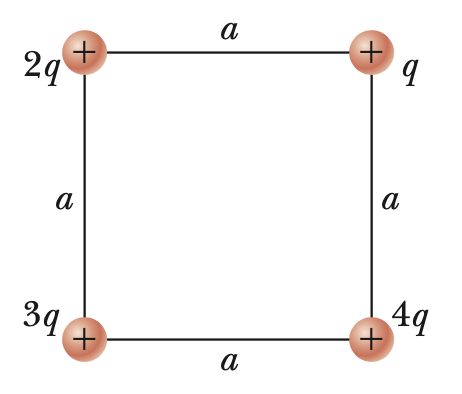
\includegraphics[scale=0.6]{qfig2-2.png}
  \caption{\textbf{문제 2}}
  \label{fig:2}
\end{figure}
\begin{itemize}
\item[(a)] 전하 $q$의 위치에서 전기장을 구하여라.
\item[(b)] $q$에 작용하는 총 정전기력을 구하여라.
\end{itemize}

\newpage

\noindent {\bf 문제 5 [20pt].} 
그림~\ref{fig:1}과 같이 $x$-축을 따라 두 전하 $q_1$과 $q_2$가 각각
$a$, $b$ 위치에 놓여 있다. 여기서 $q_2$는 음전하이다. 
\begin{itemize}
\item[(가)] $y$-축 위의 점 $P$에서 두 전하가 만드는 전기장을
  구하여라. 
\item[(나)] $|q_1|=|q_2|$, $a=b$일 때, $P$ 점에서 전기장을 구하여라. 
\item[(다)] 원점에서 $P$ 점까지의 거리가 $a$보다 매우 클 때 ($y\gg
  a$), 이 전기 쌍극자에 의한 전기장을 $P$ 점에서 구하여라. 
\end{itemize}
\begin{figure}[htp]
  \centering
  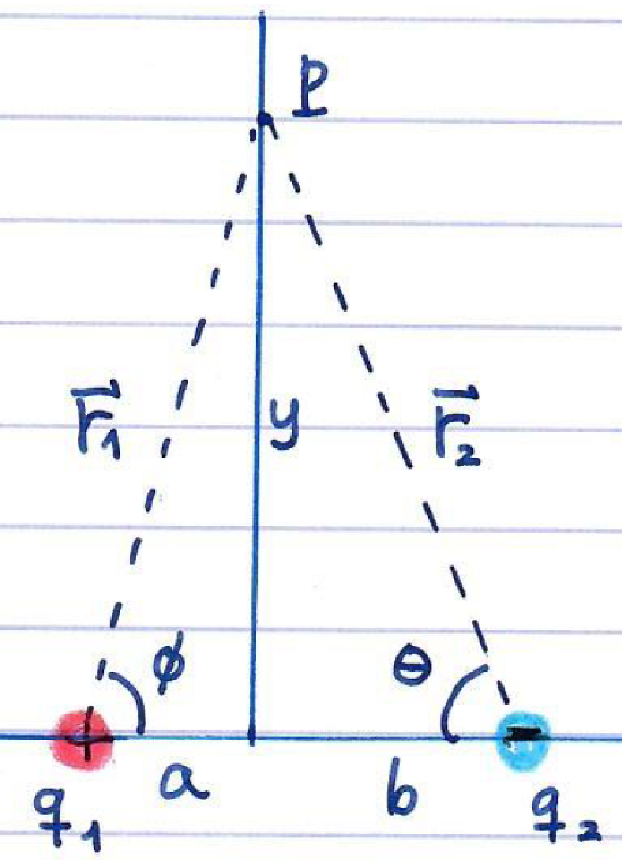
\includegraphics[scale=0.4]{Qfig20220829-1.pdf}
  \caption{\textbf{문제 5}}
  \label{fig:1}
\end{figure}
\end{document}